\documentclass[main.tex]{subfiles}

\begin{document}

\section{Issue #2557}
\label{sec:2557}

When typing display math LaTeX in a markdown note, the written LaTeX is parsed correctly but displayed incorrectly, with certain constructs having line breaks between tokens.

\subsection{Steps}
\label{subsec:steps2557}

\begin{enumerate}
\item Launch Boostnote
\item Open a new Markdown Note. Press \textit{Ctrl N} or click on the icon next to the search bar; then select Markdown Note.
\item Toggle mode to two panels in the top right corner (should be the default). Now you should have two panels open, the edit and view panels.
\item Reproduce the error. Type the following in the edit panel:
\end{enumerate}

\begin{verbatim}
        $$
        \begin{aligned}
           &P(X=x)=\binom{n}{k}P^x(1-p)^{(n-x)}\\
           &Var(X)=np(1-p)
        \end{aligned}
        $$
\end{verbatim}

\subsection{Requirements}
\label{subsec:req2557}

As of release v0.11.9 of Sep 9, and upstream master branch as of Nov 14, we get this result:

\begin{figure}[h]
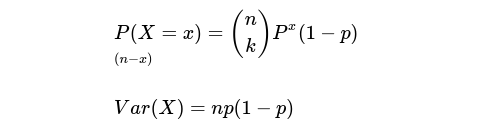
\includegraphics[scale=0.6]{images/bug1.png}
\centering
\end{figure}

However, the expected result is naturally:

\begin{figure}[h]

\includegraphics[scale=0.6]{images/bug2.png}
\centering
\end{figure}

The problem is that there is a line break where there should not be one: line breaks in display math mode are not allowed outside environments, and inside environment aligned line breaks are inserted with '\textbackslash\textbackslash', enumerating equations.

\subsection{Source Code Files}

The bug is the file:

\begin{itemize}
\item  browser/components/markdown.styl
\end{itemize}

\begin{figure}[h]
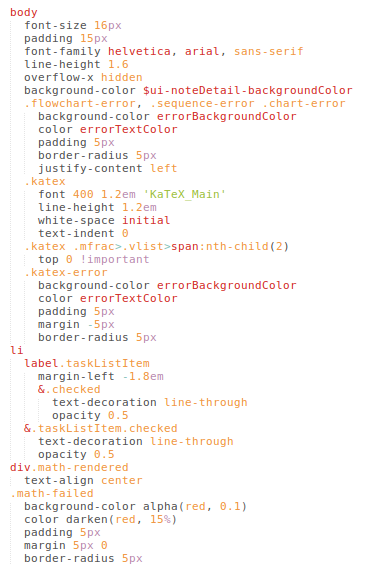
\includegraphics[scale=0.6]{images/code.png}
\centering
\end{figure}

\subsection{Source of the problem}

The problem is not in the dependency (\textbf{KaTeX}). The \textbf{KaTeX} dependency includes its own major stylesheet, which should enforce this restriction on its own display math elements. So the problem should be in some of Boostnote's own style sheets, conflicting somehow with those of \textbf{KaTeX}.

Inspecting the elements inside Boostnote (\textit{Ctrl Shift I}) suggests looking at class names \textit{.katex} and \textit{.katex-display}, as the rendered LaTeX parent element has these class names. A quick

\begin{verbatim}
        grep -rnE "\\.katex" browser/
\end{verbatim}

immediately pinpoints file markdown.styl.

\subsection{System Architecture}

A simple rundown of Boostnote's main dependencies, with emphasis on markdown-it and katex:

\begin{figure}[h]
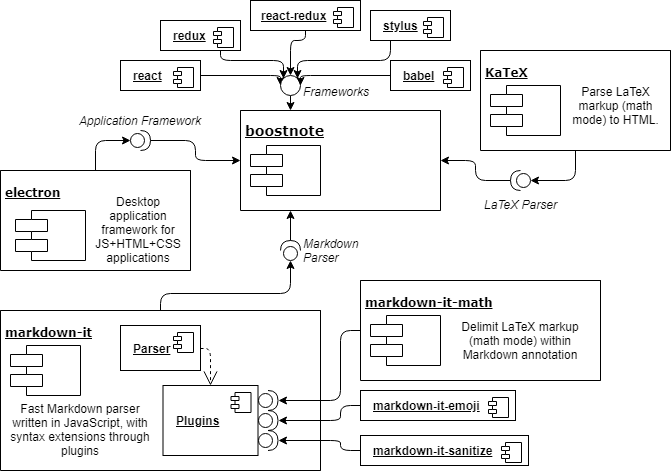
\includegraphics[scale=0.6]{images/diagram.png}
\centering
\end{figure}

\subsection{Design of the fix}

There are two ways to fix this issue. At katex.org we compare the computed styles of the LaTeX shown right on the front page to those of Boostnote applied to the same LaTeX elements. In particular we looked at attributes like display, textalign, and overflow-wrap. We concluded quickly that the problem was in the attribute white-space, whose value was reset to initial in Boostnote (meaning normal), instead of nowrap.\\

Changing this attribute to nowrap will have unintended side effects (no wrapping in inline math mode), so the problem, albeit simple, will require further testing. The most likely solution will involve demoting selector body .katex to .katex-inline or removing the attribute, or even removing the .katex rules altogether.

\nocite{*}

\end{document}